\begin{frame}{Malha de Biomas}
    \begin{itemize} \setlength\itemsep{1em}
        \item As regiões de biomas tem áreas quadradas de lado $b$;
    \end{itemize}
\end{frame}

\begin{frame}{Regiões dos Biomas}
    \begin{figure}[H]
        \centering
        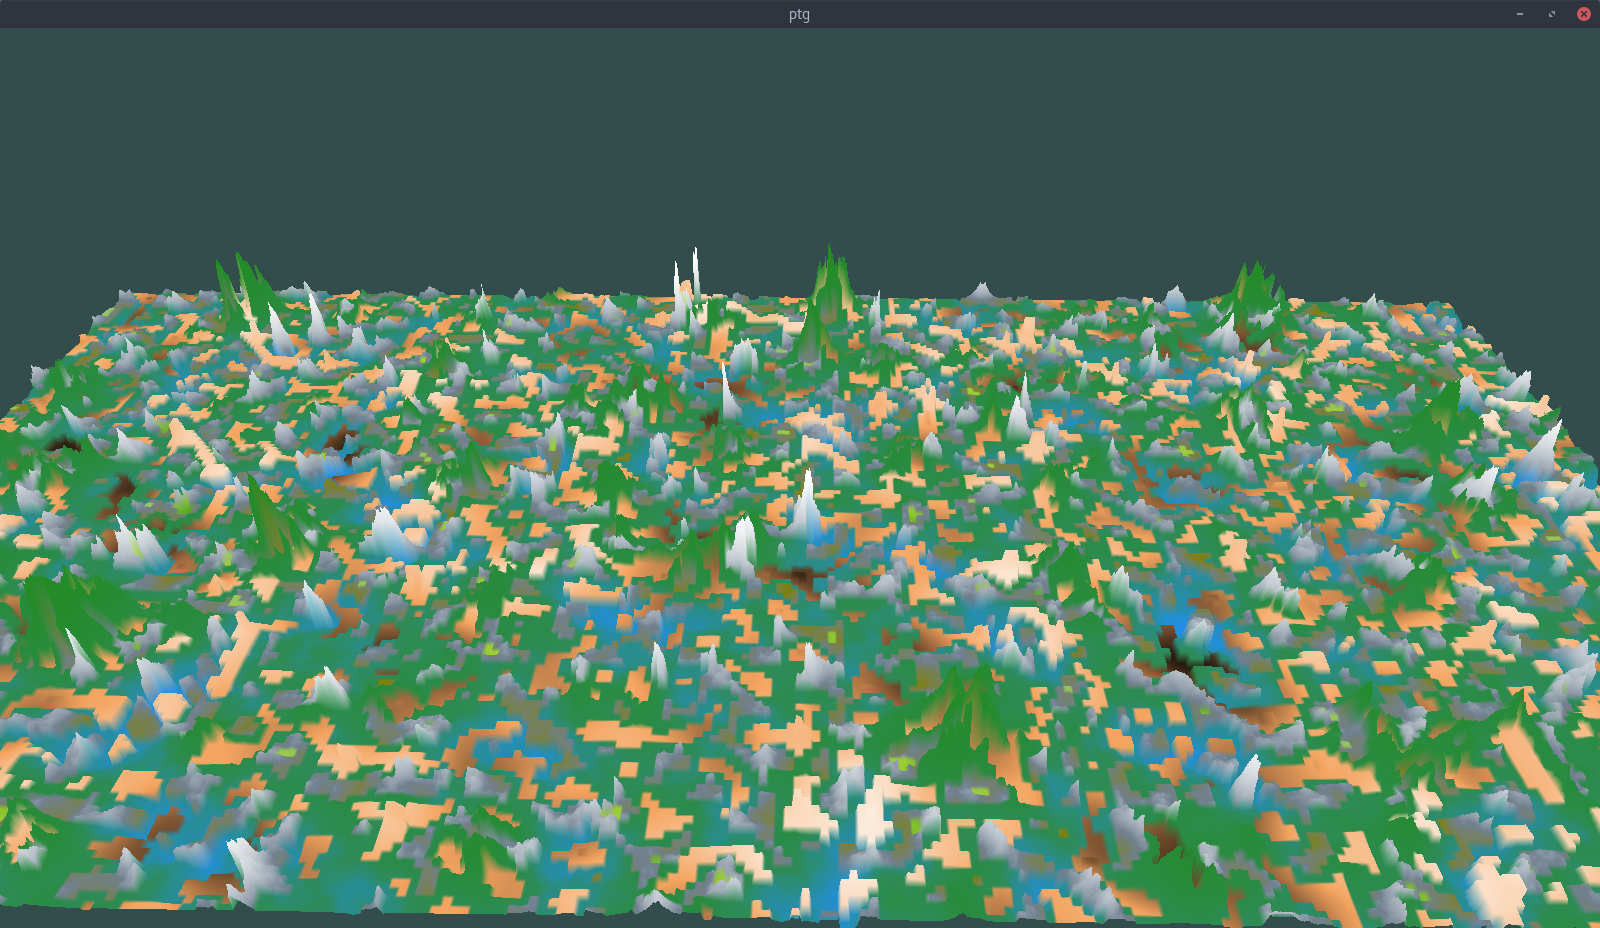
\includegraphics[width=.9\textwidth]{img/re2bfb/b/16f4.png}
        \caption{Regiões com $b = 16$.}
        \label{fig:img_re2bfb_b_16f4}
    \end{figure}
    
    
\end{frame}

\begin{frame}{Malha de Biomas}
    \begin{figure}[H]
        \centering
        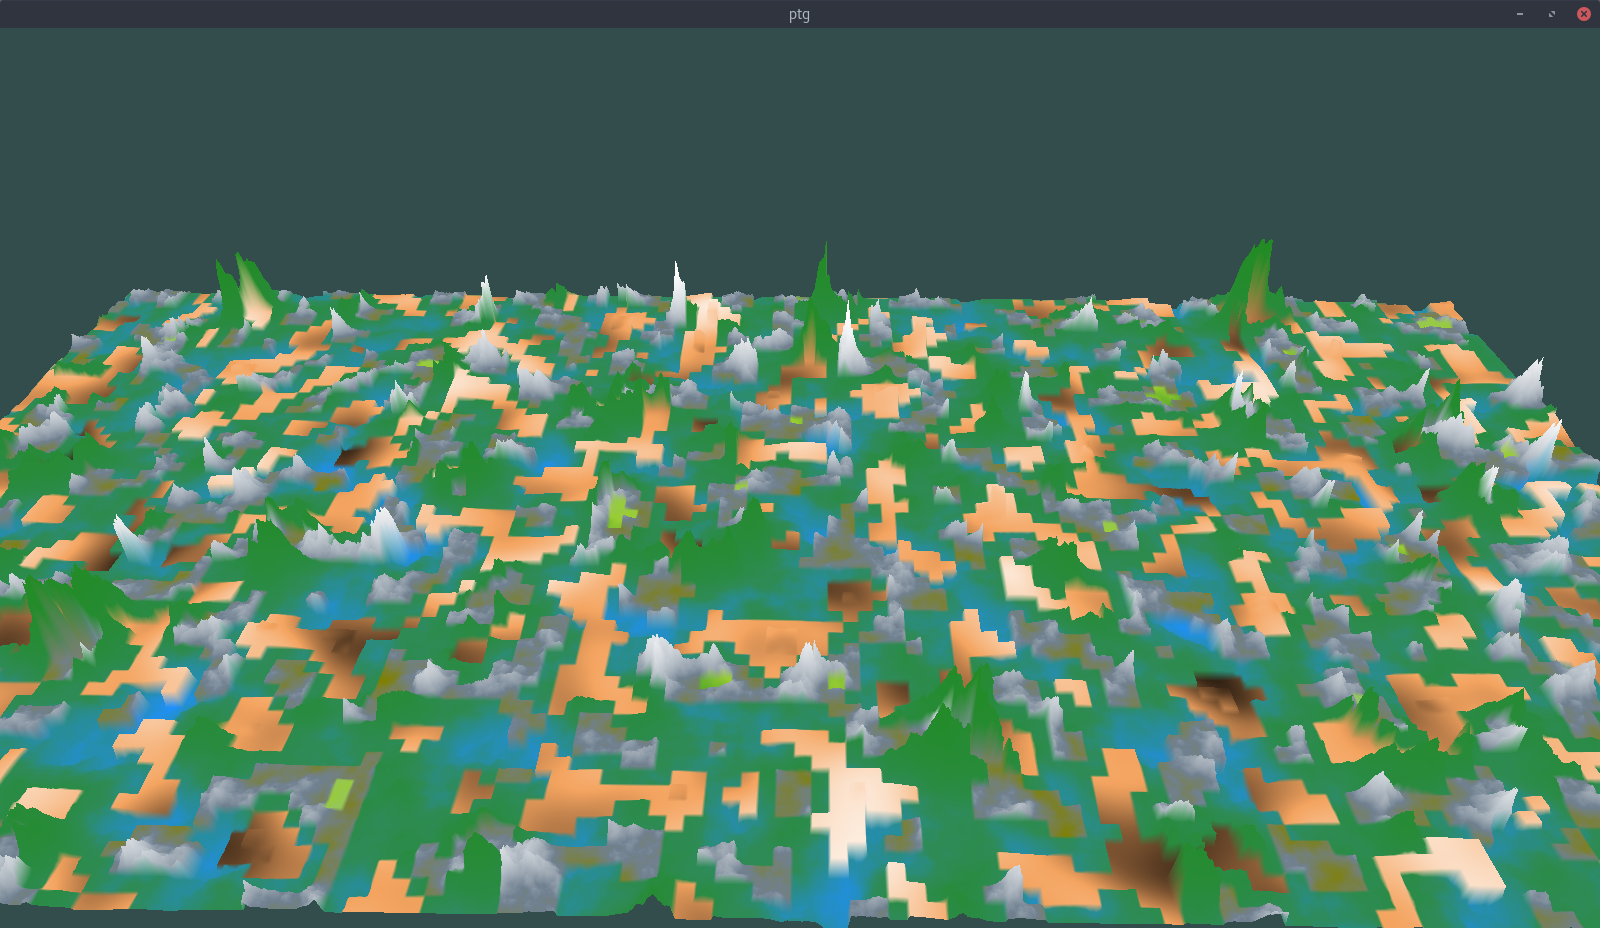
\includegraphics[width=.9\textwidth]{img/re2bfb/b/32f4.png}
        \caption{Regiões com $b = 32$.}
        \label{fig:img_re2bfb_b_32f4}
    \end{figure}
    
    
\end{frame}

\begin{frame}{Malha de Biomas}
    \begin{figure}[H]
        \centering
        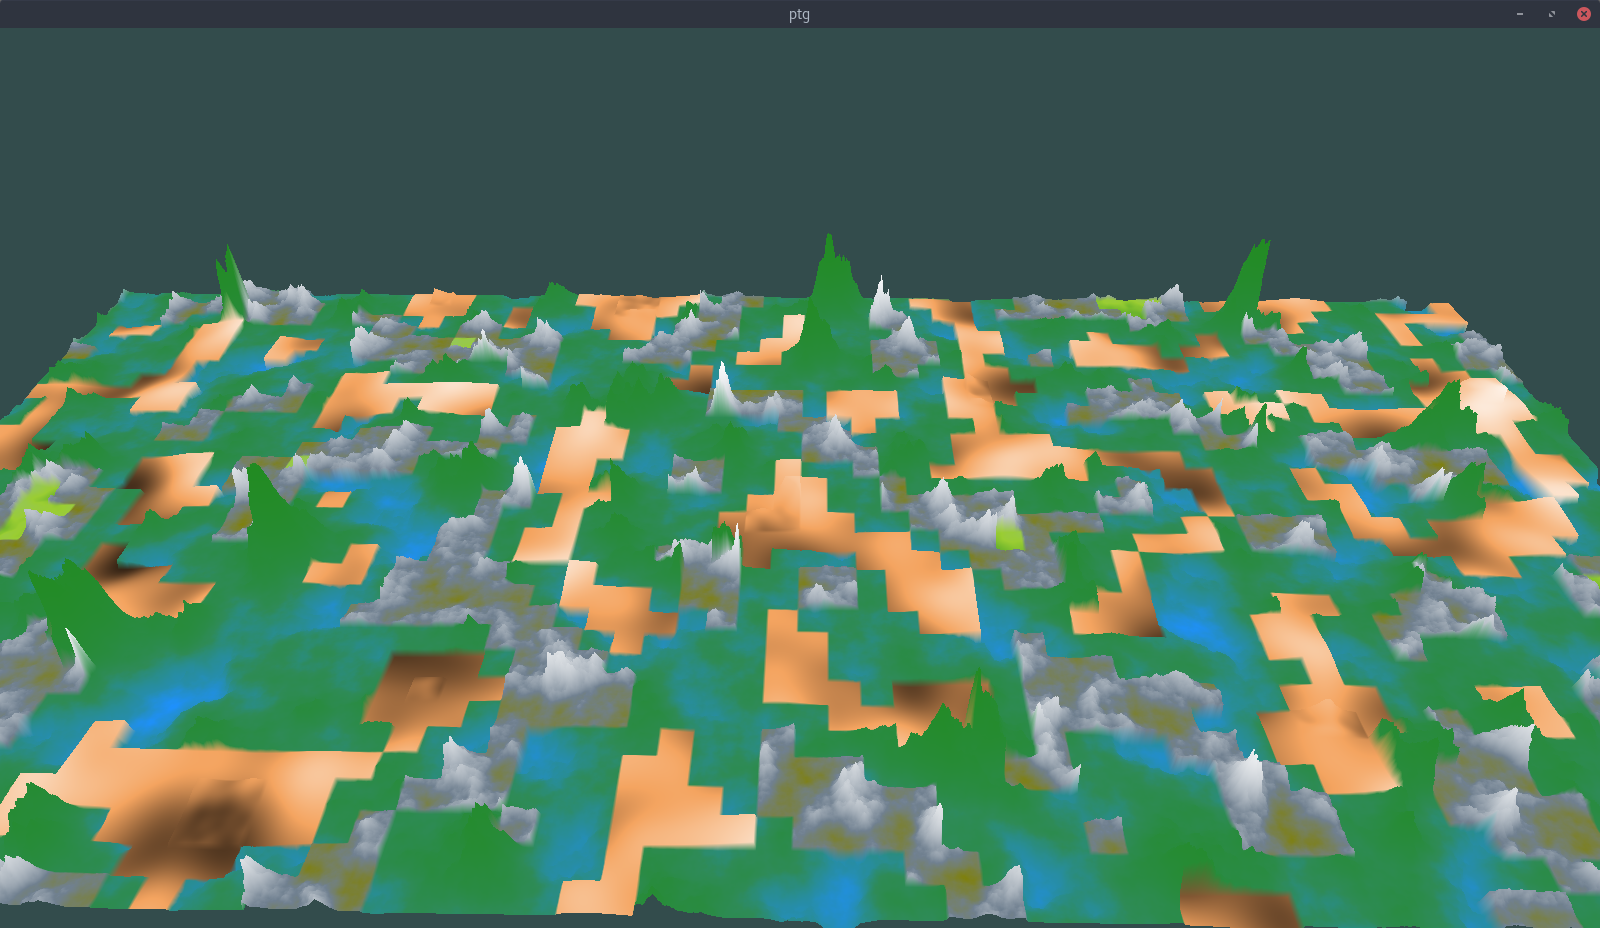
\includegraphics[width=.9\textwidth]{img/re2bfb/b/64f4.png}
        \caption{Regiões com $b = 64$.}
        \label{fig:img_re2bfb_b_64f4}
    \end{figure}
    
    
\end{frame}

\begin{frame}{Malha de Biomas}
    \begin{figure}[H]
        \centering
        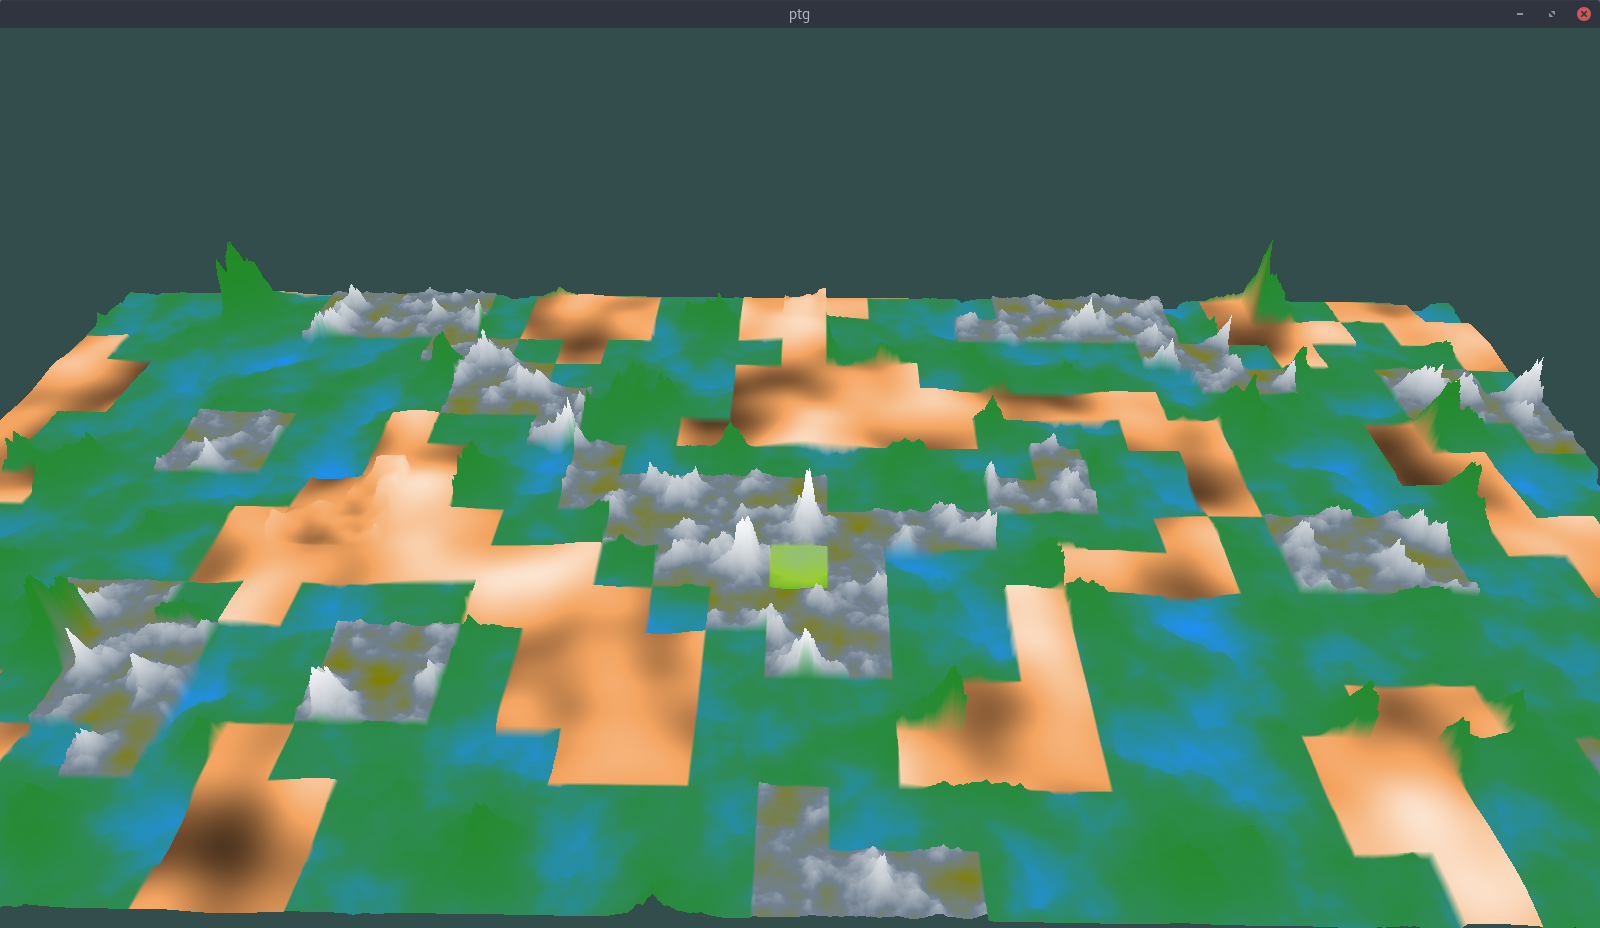
\includegraphics[width=.9\textwidth]{img/re2bfb/b/128f4.png}
        \caption{Regiões com $b = 128$.}
        \label{fig:img_re2bfb_b_128f4}
    \end{figure}
    
    
\end{frame}

\begin{frame}{Malha de Biomas}
    \begin{figure}[H]
        \centering
        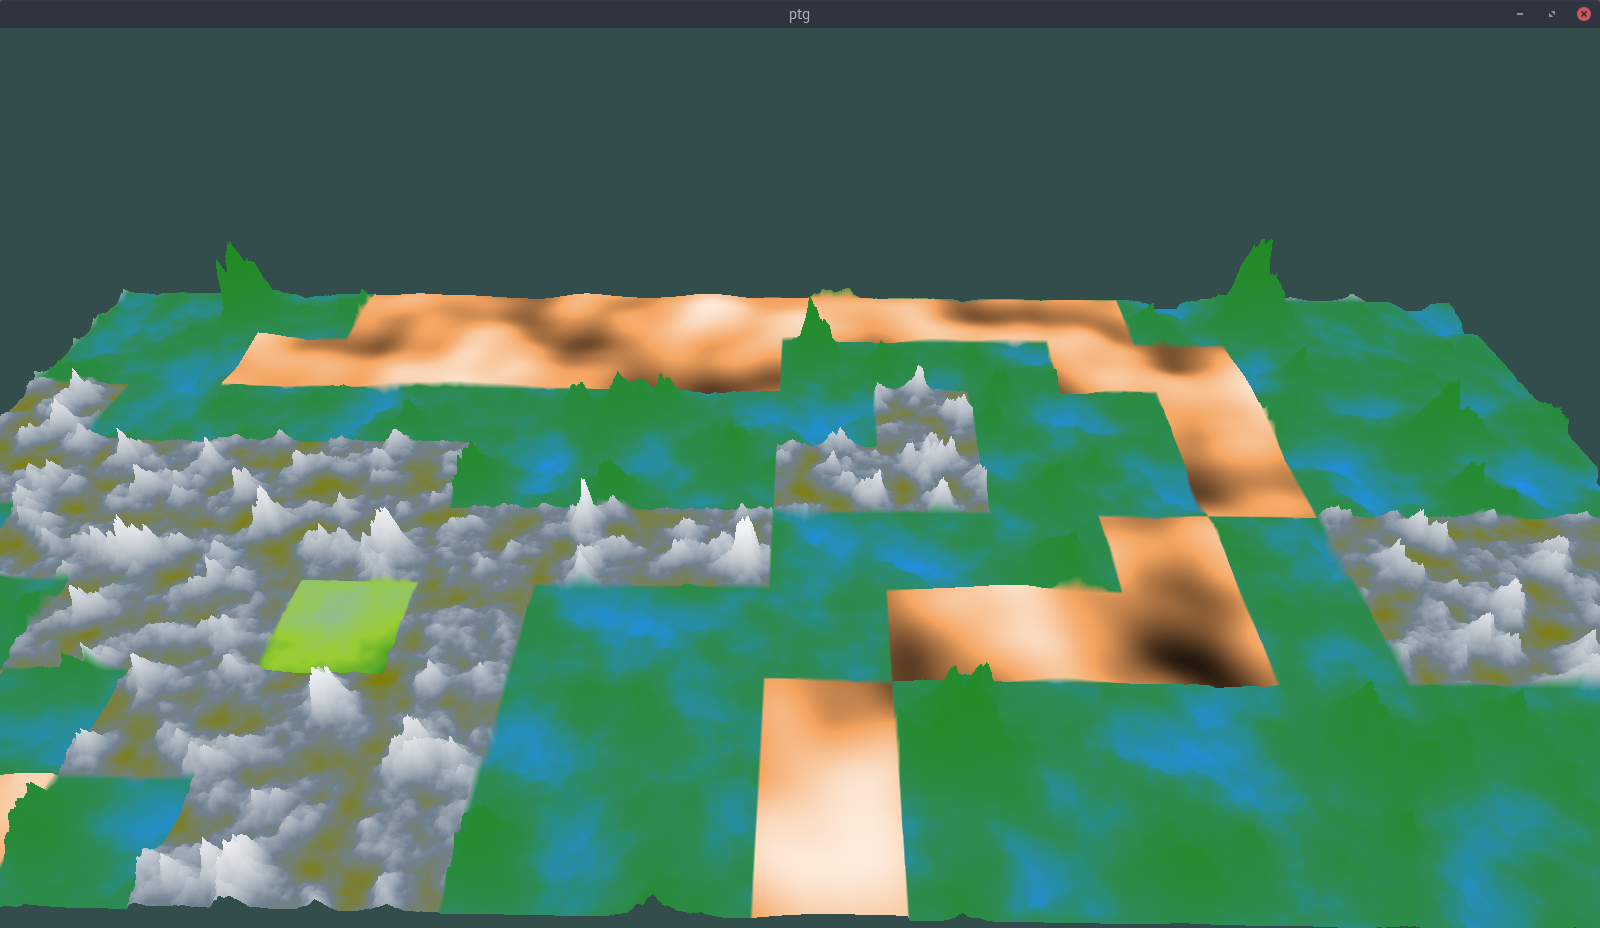
\includegraphics[width=.9\textwidth]{img/re2bfb/b/256f4.png}
        \caption{Regiões com $b = 256$.}
        \label{fig:img_re2bfb_b_256f4}
    \end{figure}
    
    
\end{frame}

\begin{frame}{Malha de Biomas}
    \begin{figure}[H]
        \centering
        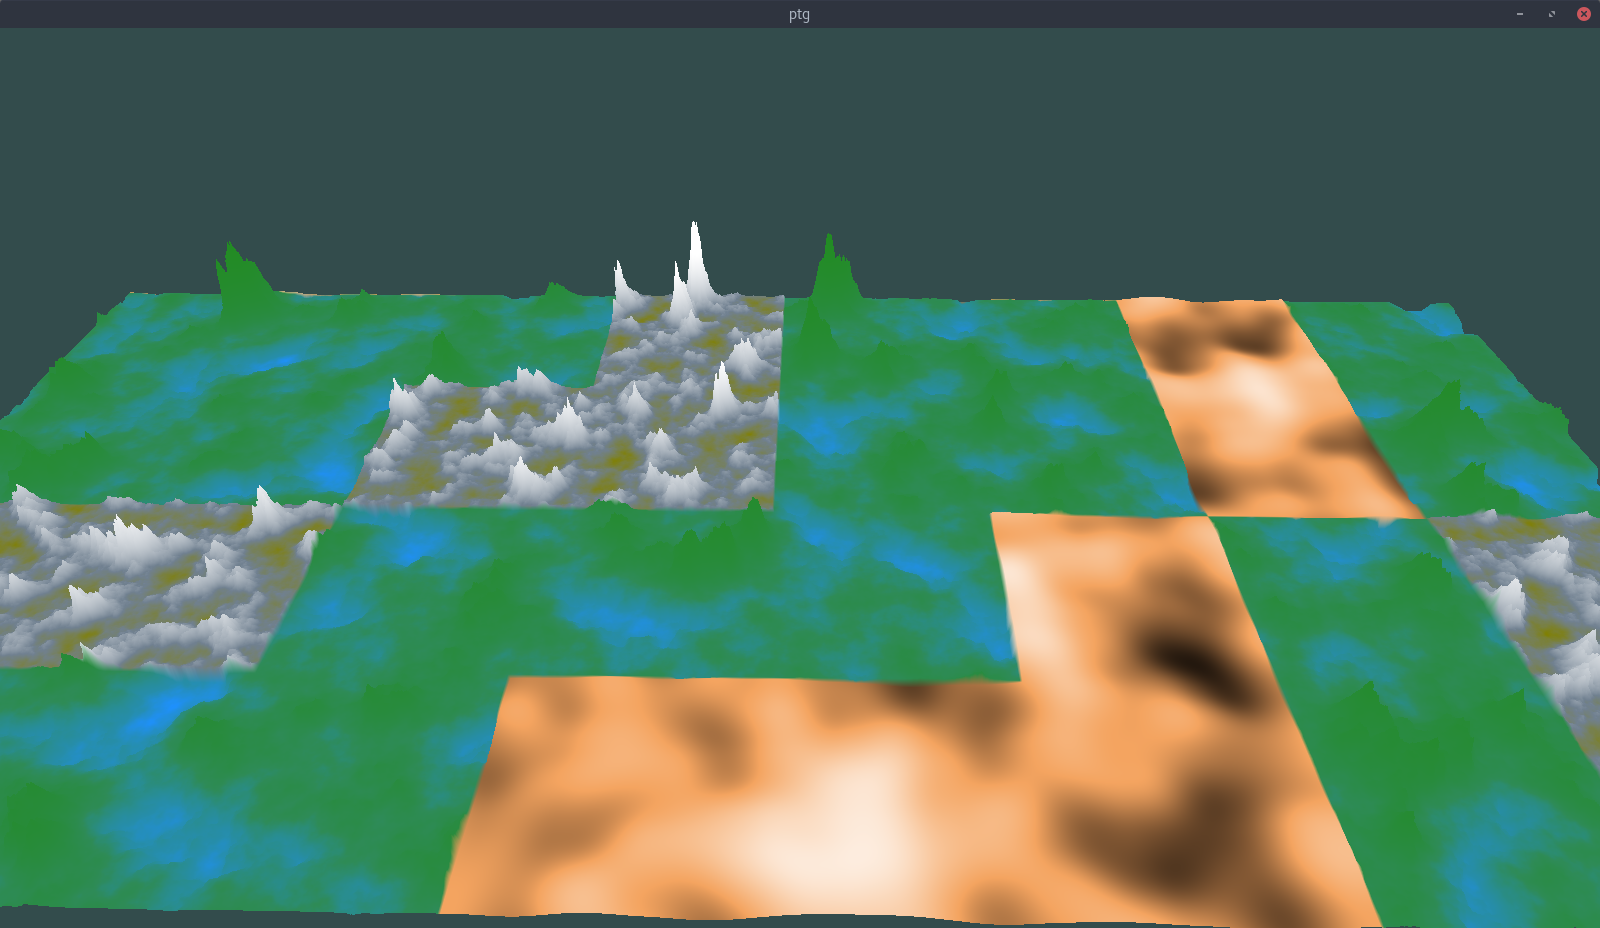
\includegraphics[width=.9\textwidth]{img/re2bfb/b/512f4.png}
        \caption{Regiões com $b = 512$.}
        \label{fig:img_re2bfb_b_512f4}
    \end{figure}
    
    
\end{frame}

\begin{frame}{Malha de Biomas}
    \begin{itemize} \setlength\itemsep{1em}
        \item Cada região usa a chave $(dxs, dzs)$ como parâmetro de ruído para definir seu bioma
        \item A frequência com que mudam os biomas ao longo da malha é $1/fb$
        \item Vantagem de usar ruído para distribuir os biomas
        \begin{figure}[H]
            \centering
            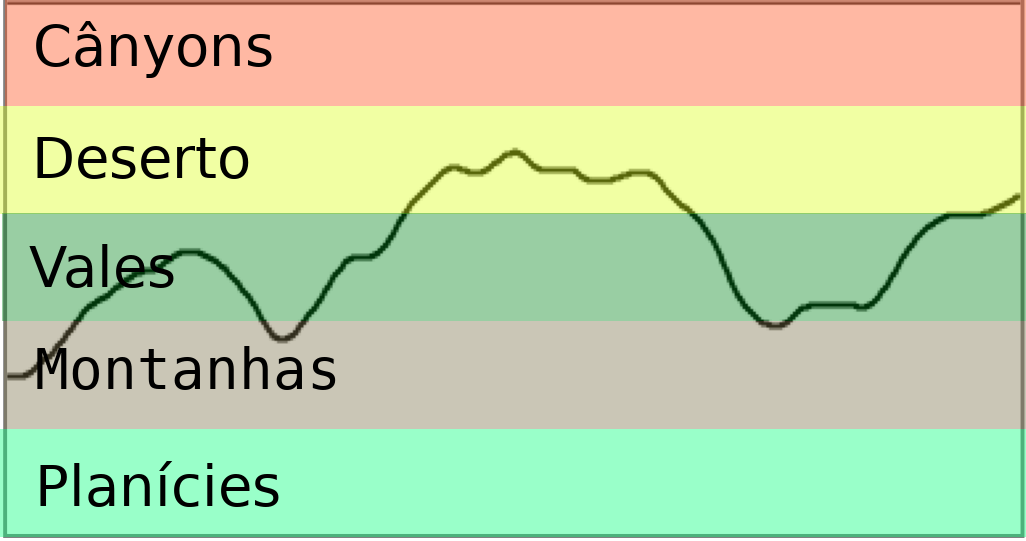
\includegraphics[width=.6\textwidth]{img/re2bfb/distnoise.png}
            \caption{Distribuições de biomas, ruído ao fundo \cite{shiffman2012nature}.}
            \label{fig:img_re2bfb_distnoise}
        \end{figure}
    \end{itemize}
\end{frame}

\begin{frame}{Malha de Biomas}
    \begin{figure}[H]
        \centering
        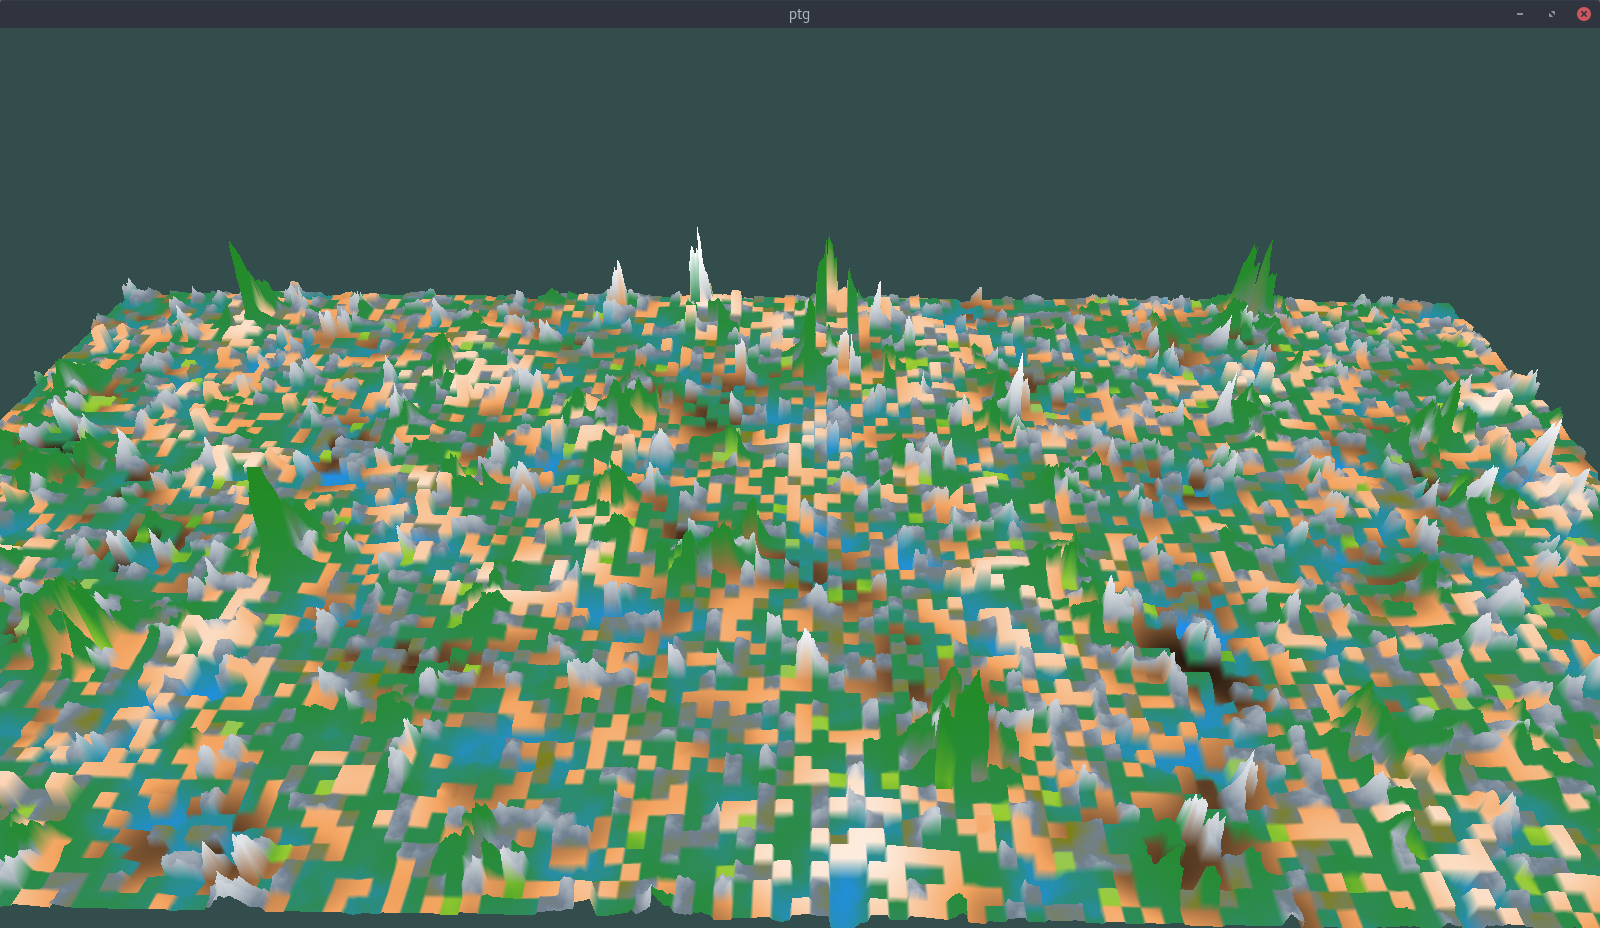
\includegraphics[width=.9\textwidth]{img/re2bfb/fb/05b32.png}
        \caption{Regiões com $b = 32$ e $fb = 0.5$.}
        \label{fig:img_re2bfb_fb_05b32}
    \end{figure}
    
    
\end{frame}

\begin{frame}{Malha de Biomas}
    \begin{figure}[H]
        \centering
        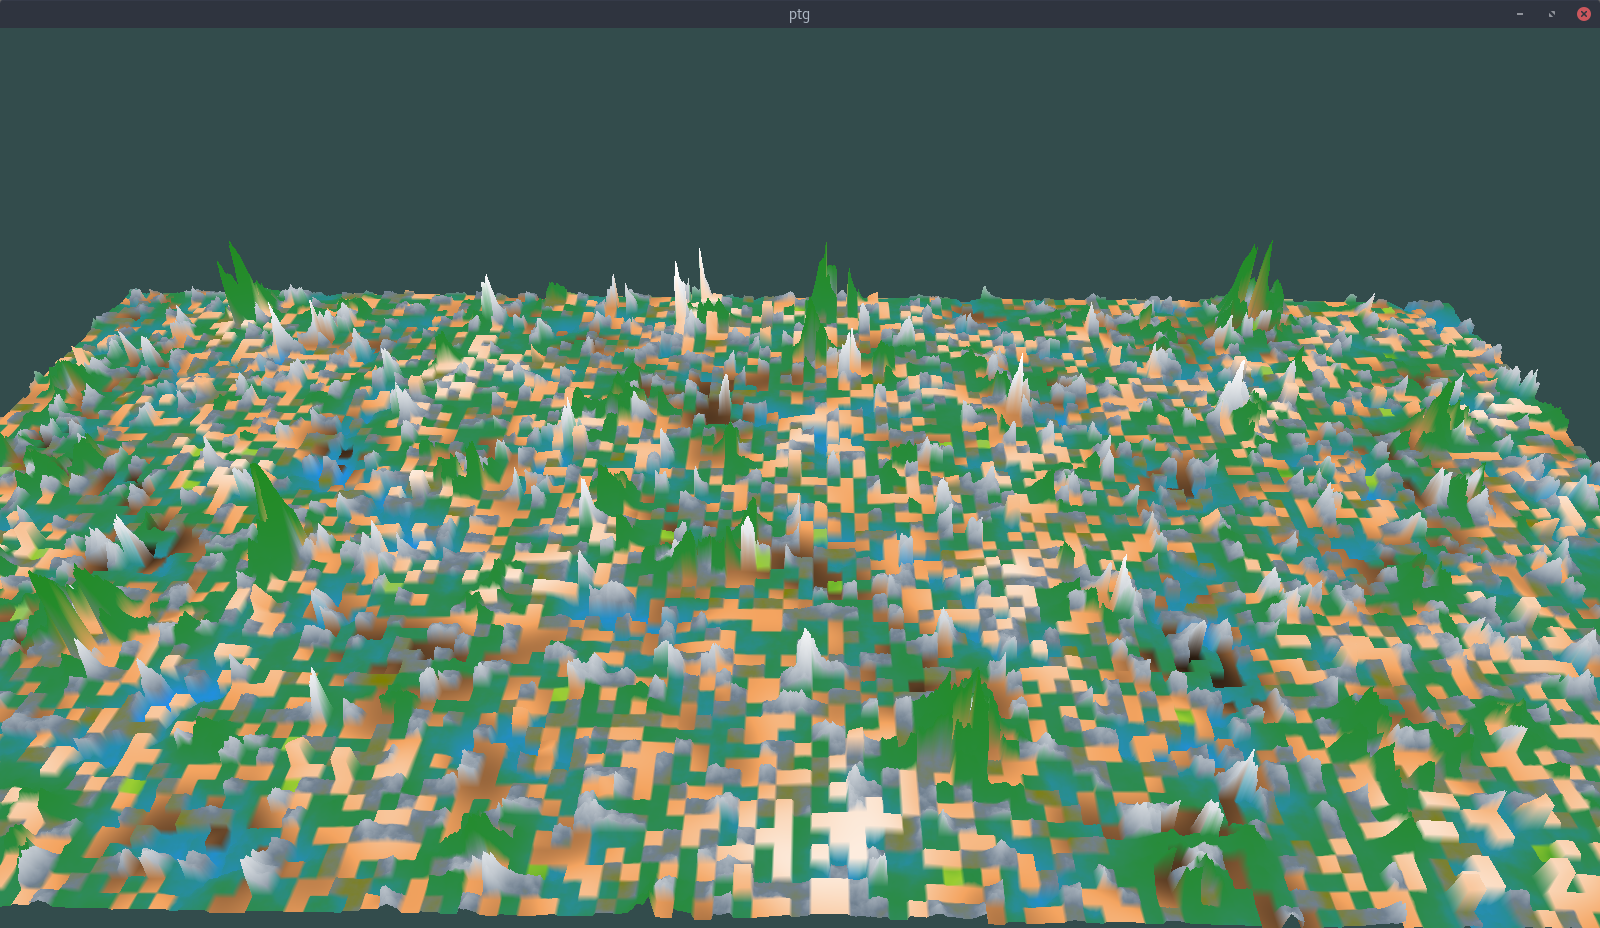
\includegraphics[width=.9\textwidth]{img/re2bfb/fb/1b32.png}
        \caption{Regiões com $b = 32$ e $fb = 1$.}
        \label{fig:img_re2bfb_fb_1b32}
    \end{figure}
    
    
\end{frame}

\begin{frame}{Malha de Biomas}
    \begin{figure}[H]
        \centering
        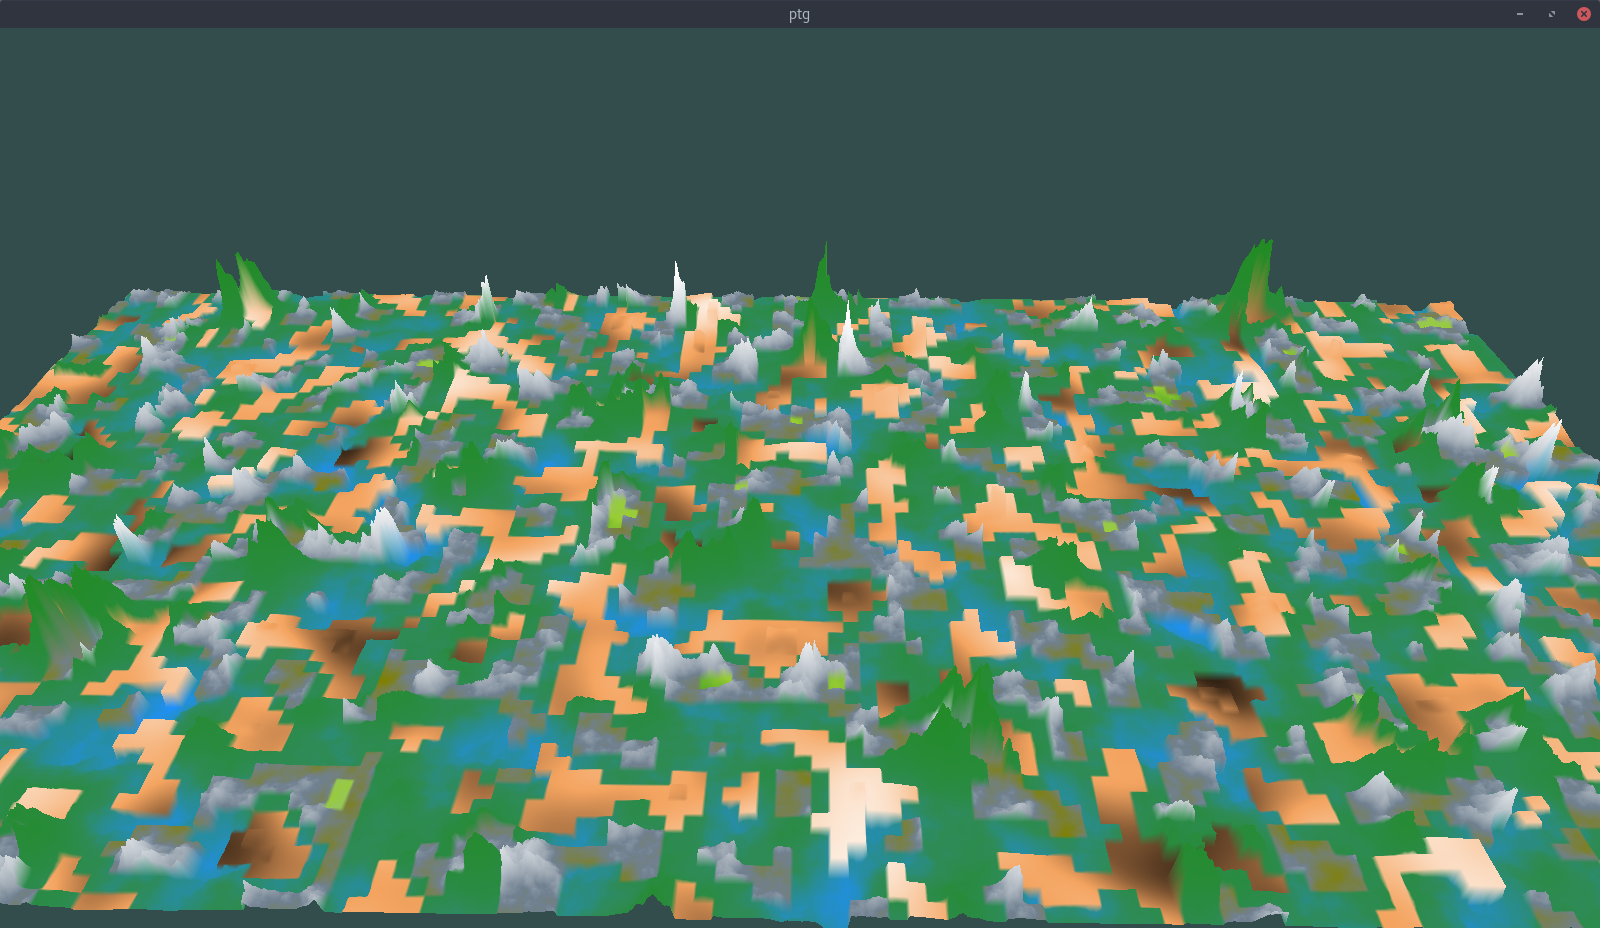
\includegraphics[width=.9\textwidth]{img/re2bfb/fb/4b32.png}
        \caption{Regiões com $b = 32$ e $fb = 4$.}
        \label{fig:img_re2bfb_fb_4b32}
    \end{figure}
    
    
\end{frame}

\begin{frame}{Malha de Biomas}
    \begin{figure}[H]
        \centering
        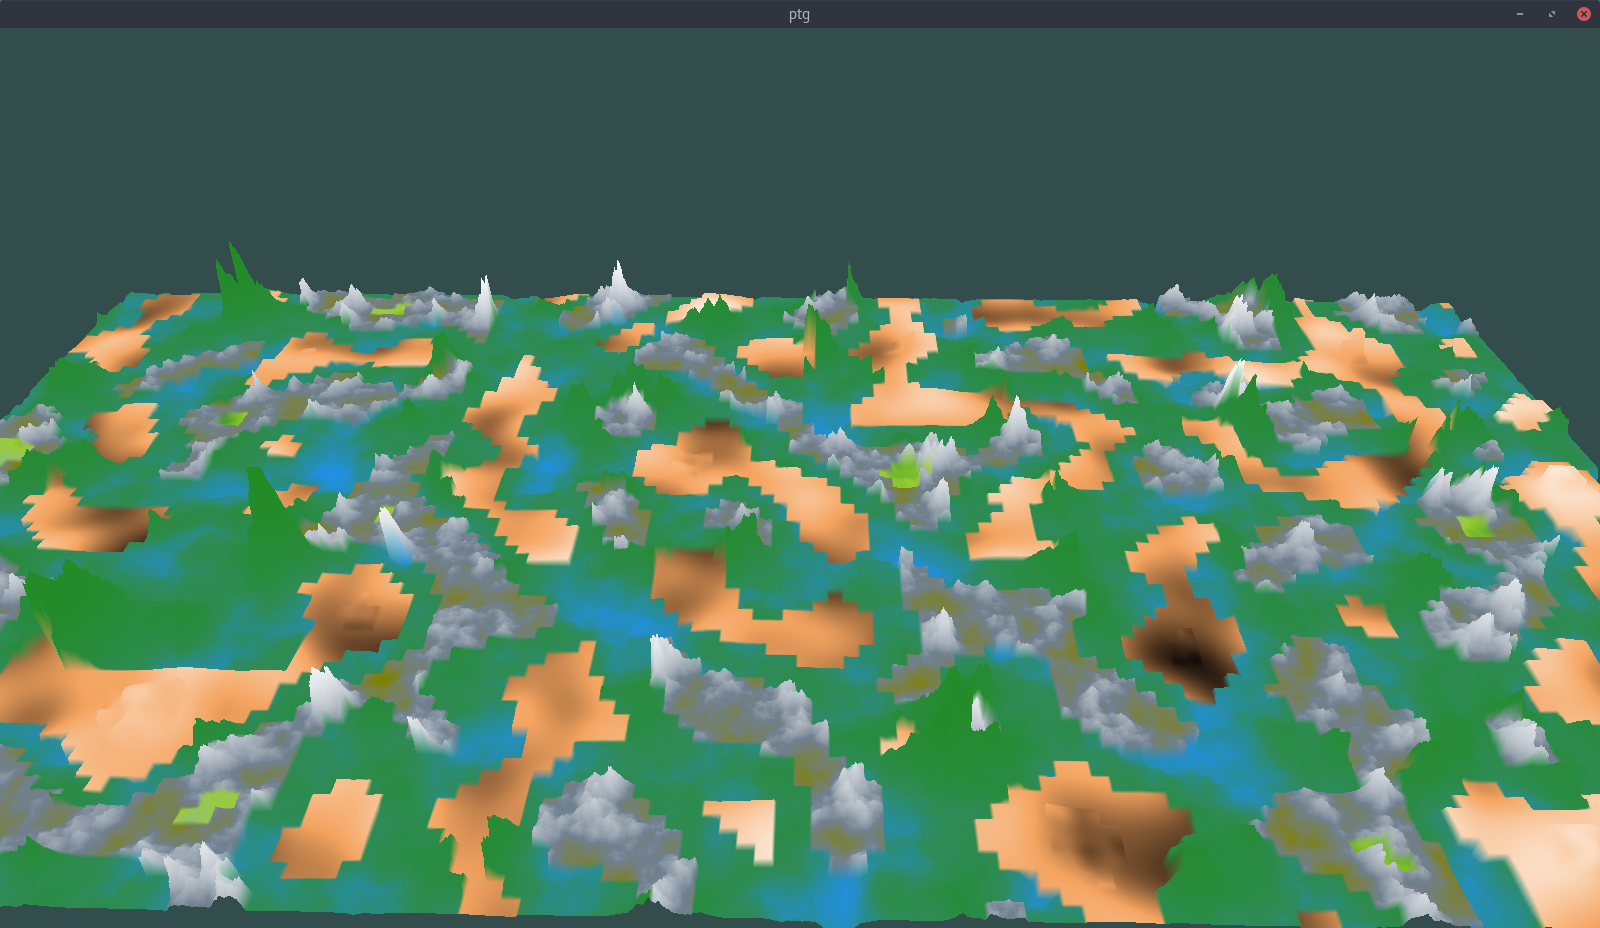
\includegraphics[width=.9\textwidth]{img/re2bfb/fb/8b32.png}
        \caption{Regiões com $b = 32$ e $fb = 8$.}
        \label{fig:img_re2bfb_fb_8b32}
    \end{figure}
    
    
\end{frame}

\begin{frame}{Malha de Biomas}
    \begin{figure}[H]
        \centering
        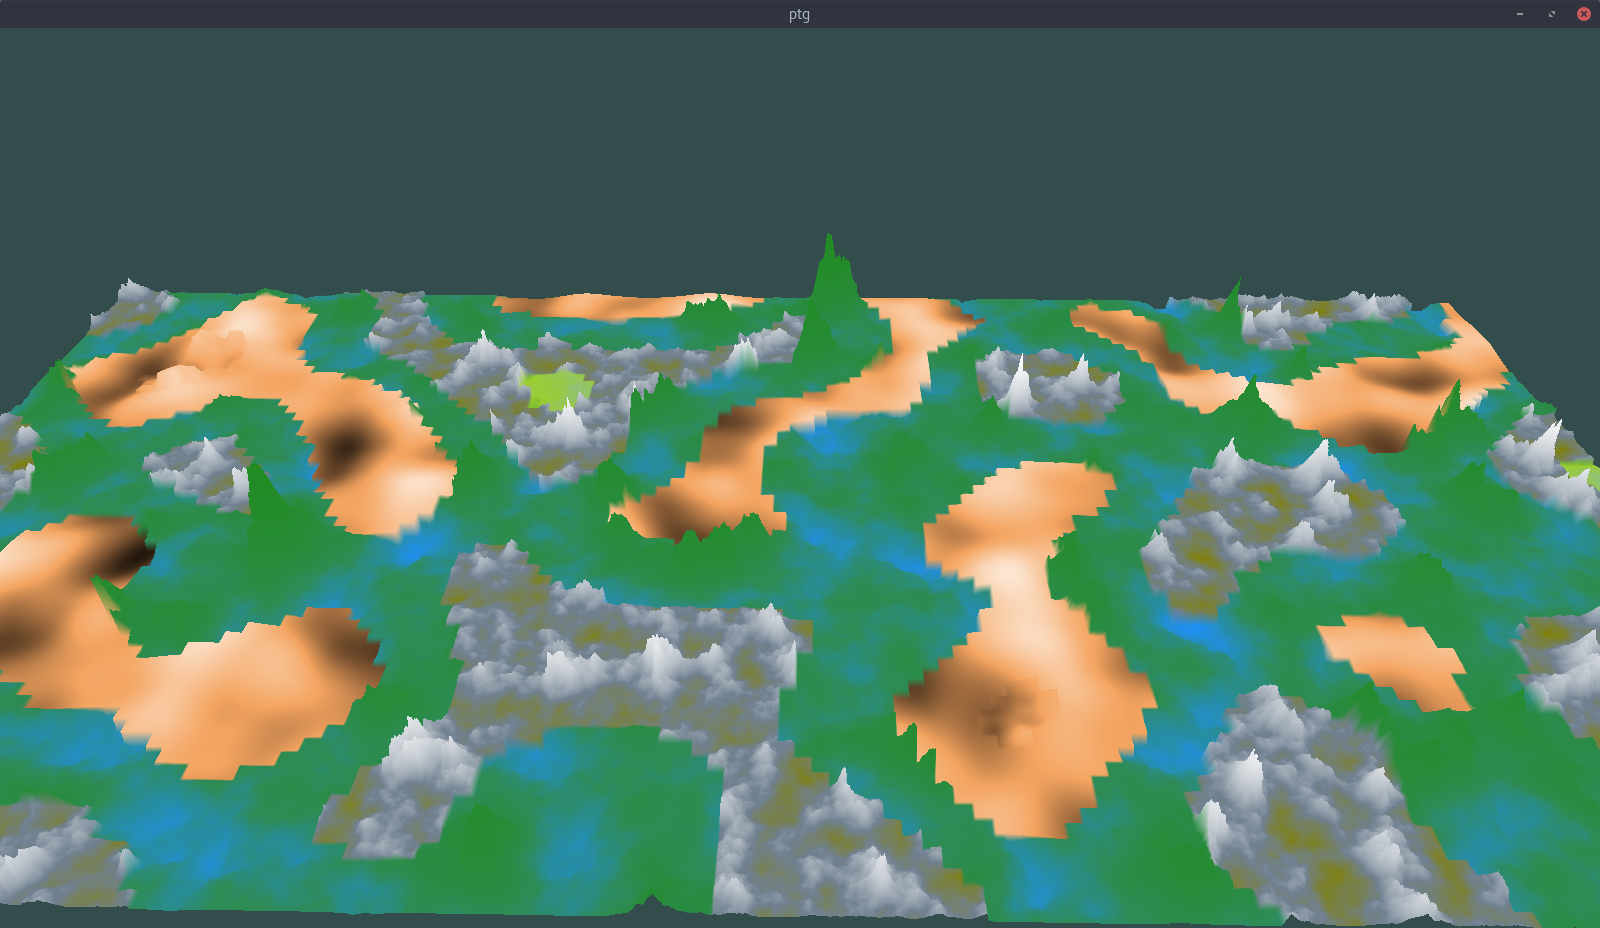
\includegraphics[width=.9\textwidth]{img/re2bfb/fb/16b32.png}
        \caption{Regiões com $b = 32$ e $fb = 16$.}
        \label{fig:img_re2bfb_fb_16b32}
    \end{figure}
    
    
\end{frame}

\begin{frame}{Malha de Biomas}
    \begin{figure}[H]
        \centering
        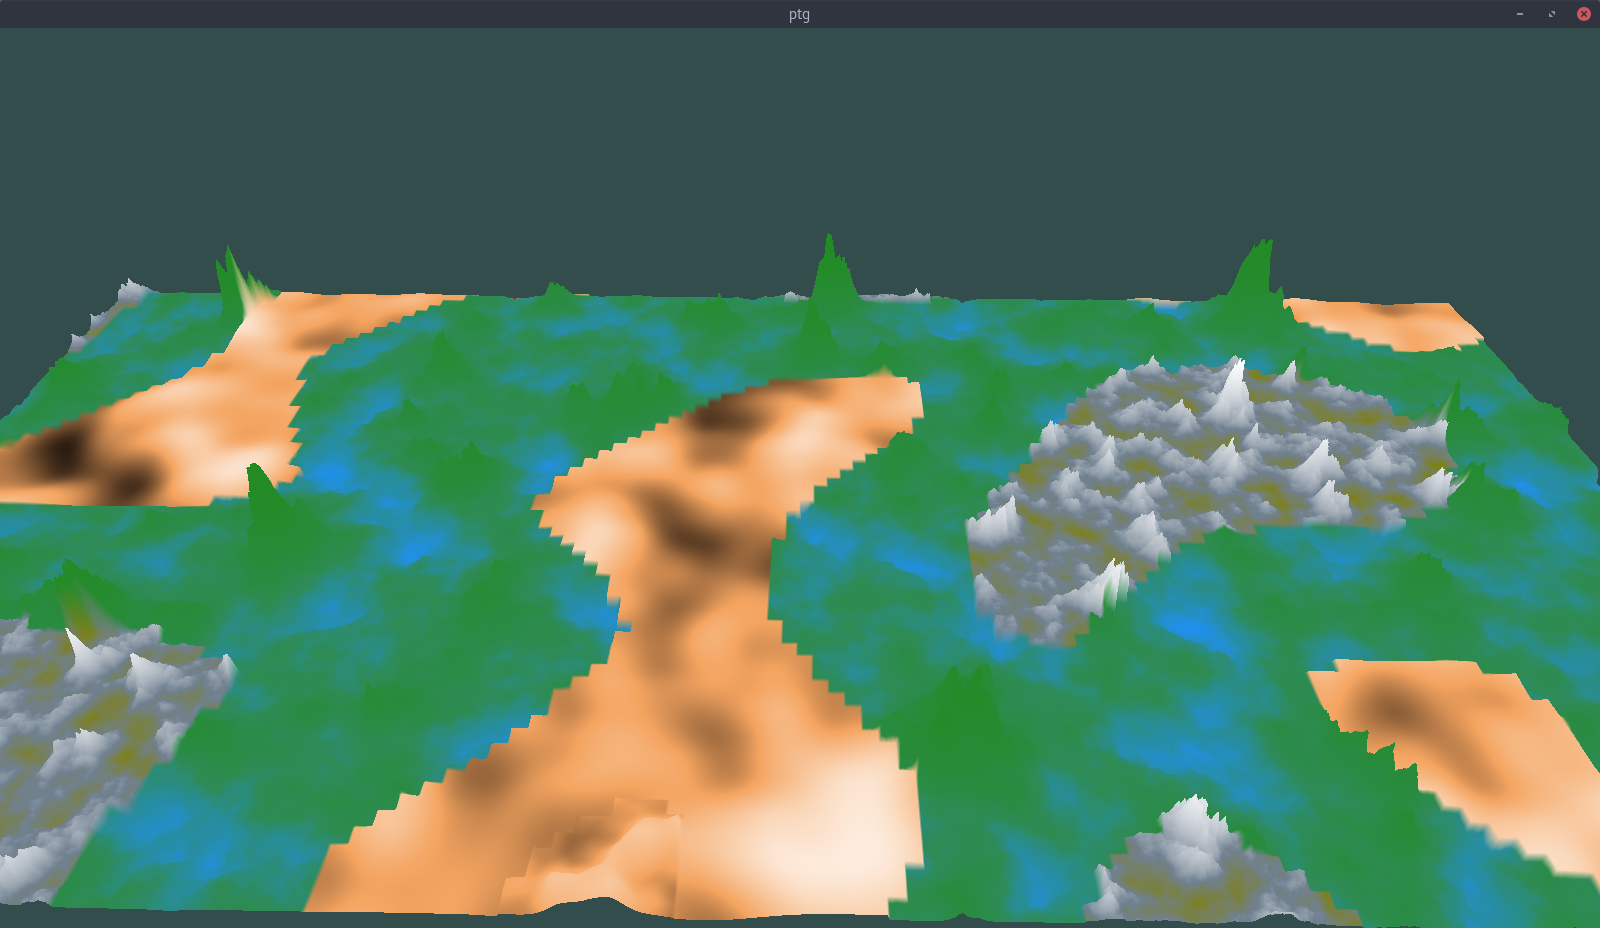
\includegraphics[width=.9\textwidth]{img/re2bfb/fb/32b32.png}
        \caption{Regiões com $b = 32$ e $fb = 32$.}
        \label{fig:img_re2bfb_fb_32b32}
    \end{figure}
    
    
\end{frame}

\begin{frame}{Malha de Biomas}
    \begin{figure}[H]
        \centering
        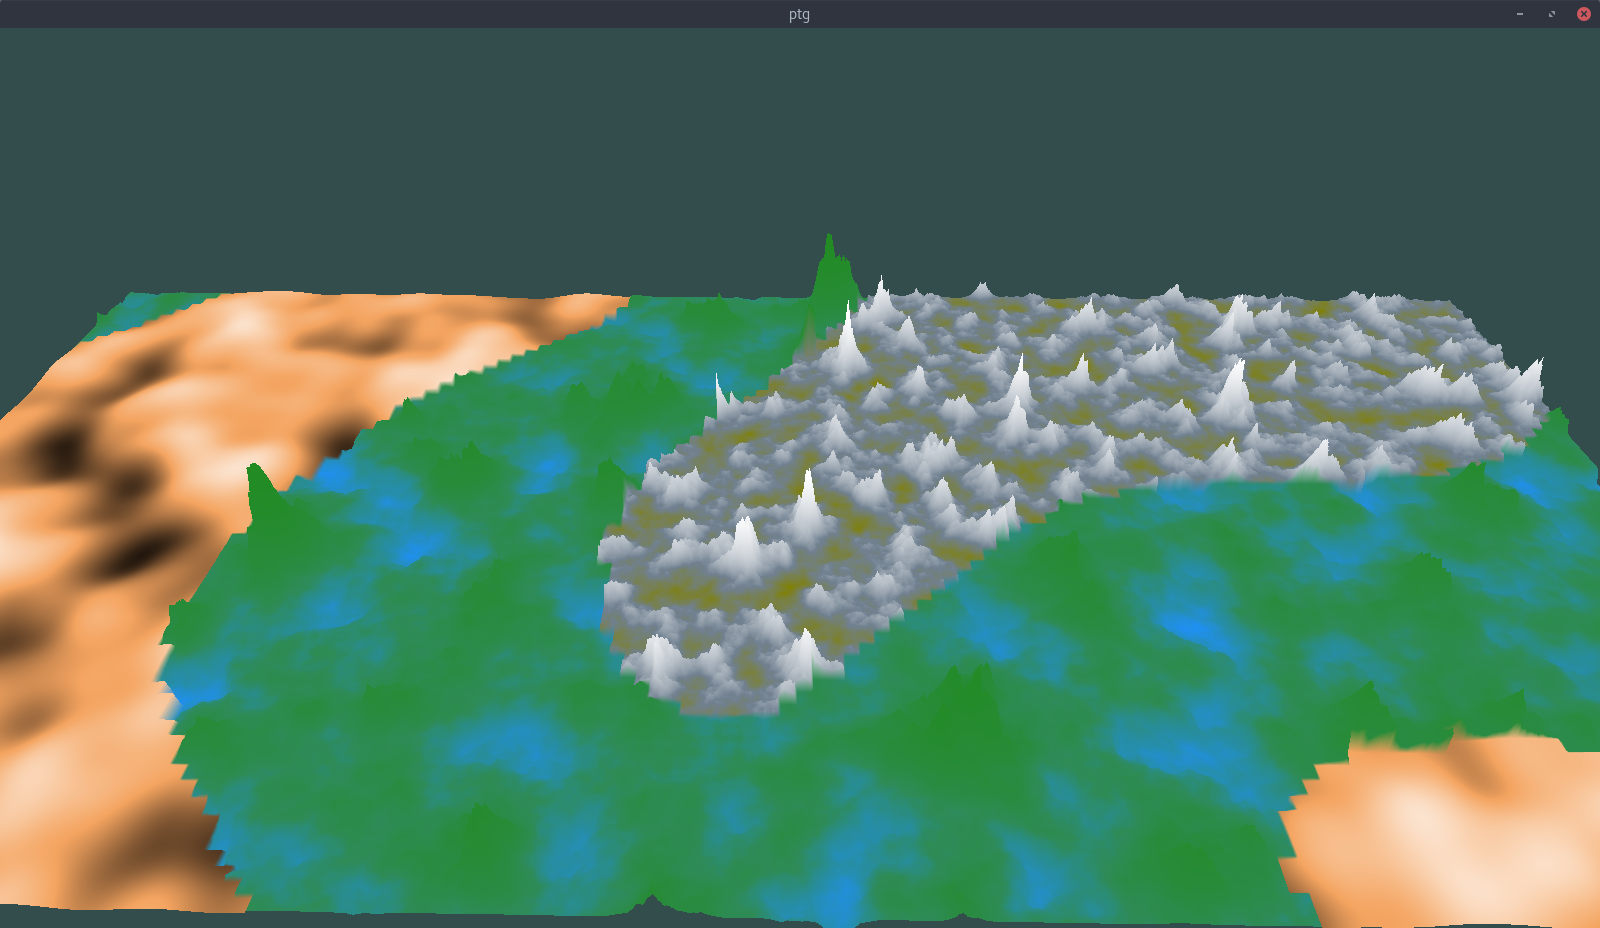
\includegraphics[width=.9\textwidth]{img/re2bfb/fb/64b32.png}
        \caption{Regiões com $b = 32$ e $fb = 64$.}
        \label{fig:img_re2bfb_fb_64b32}
    \end{figure}
    
    
\end{frame}